\documentclass[a4paper,11pt]{article}
\usepackage{booktabs} % Provides professional-quality horizontal rules
\usepackage{float} % Required for [H] placement
\usepackage{tikz}
\usepackage{hyperref}

\hypersetup{
    colorlinks=true,    % True removes the default red/green border boxes
    linkcolor=blue,     % Colors internal links (like the TOC) blue
    urlcolor=cyan       % Colors external URLs cyan
}

\newcommand{\newpagex}{
    \newpage
    \vspace*{-7\baselineskip} % Pulls text up by one line
}

\author{Hectron} 

\title{Minimum Substring}

\begin{document}

% generates the title
\maketitle

% insert the table of contents
\tableofcontents

% seperate body and table of contents 
\newpagex
    \noindent

\section{Description}
    
    Given two strings s and t of lengths m and n respectively, return the minimum window of s such that every character in  in t (including duplicates) is included in the window.

    \begin{itemize}
    \item \textbf{Input:} \newline \textmd{s = ``ADOBECODEBANC''} \newline \textmd{t = ``ABC''}
    \item \textbf{Output}: \newline  \textmd{``BANC''}
    \item \textbf{Explanation}: \newline  \textmd{The minimum window substring ``BANC'' includes `A', `B', and `C' from string t.}
    \end{itemize}

\section{Function/Method Declaration}
    \footnotesize

    \begin{verbatim}
        class Solution {
        
        public:

            std::string minWindow\(std::string s, std::string t);

        }

    \end{verbatim}


\section{How to solve}
    


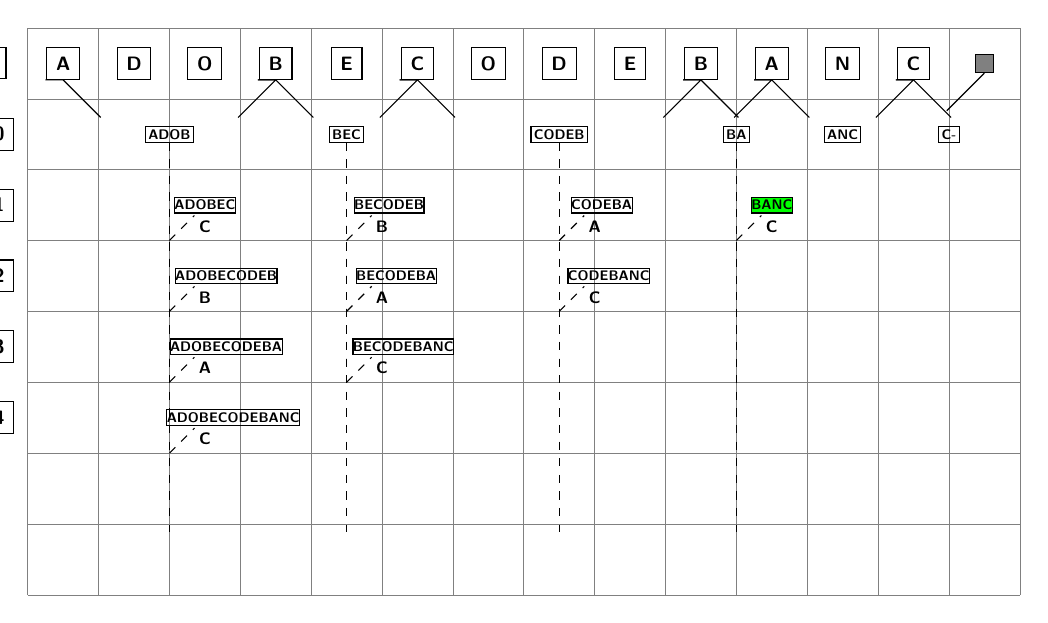
\begin{tikzpicture}[node distance=1.0cm , trim left=0cm, scale=0.9]


    \draw[help lines, opacity=1] (0,0) grid (14,8 );

    \node (p)  at ( -1.0, 7.5) [draw, font=\fontsize{7}{9}\selectfont\sffamily\bfseries] {sequence};
    \node (p2)  at ( -1.0, 6.5) [draw, font=\fontsize{7}{9}\selectfont\sffamily\bfseries] {accNodes0};
    \node (p3)  at ( -1.0, 5.5) [draw, font=\fontsize{7}{9}\selectfont\sffamily\bfseries] {accNodes1};
    \node (p3)  at ( -1.0, 4.5) [draw, font=\fontsize{7}{9}\selectfont\sffamily\bfseries] {accNodes2};
    \node (p4)  at ( -1.0, 3.5) [draw, font=\fontsize{7}{9}\selectfont\sffamily\bfseries] {accNodes3};
    \node (p5)  at ( -1.0, 2.5) [draw, font=\fontsize{7}{9}\selectfont\sffamily\bfseries] {accNodes4};

    \node (seq0)  at ( 0.5, 7.5 )[draw, font=\fontsize{7}{9}\selectfont\sffamily\bfseries] {A};
    % \node (seq0)  at ( 0.5, 7.5) \drawnode{} {A};
    \draw[-] (seq0.south) -- ++(-0.25, 0 ) -- (seq0.south) -- ++(-45 : 0.75cm ) ;

    \node (seq1)  at ( 1.5, 7.5) [draw, font=\fontsize{7}{9}\selectfont\sffamily\bfseries] {D};
    % \draw[-] (seq1.south) -- ++(-0.25, 0 )  -- (seq1.south) -- ++(225 : 0.75cm ) ;
    % \draw[-] (seq1.south) -- ++(-0.25, 0 )  -- (seq1.south) -- ++(-45 : 0.75cm ) ;

    \node (seq2)  at ( 2.5, 7.5) [draw, font=\fontsize{7}{9}\selectfont\sffamily\bfseries] {O};
    % \draw[-] (seq2.south) -- ++(-0.25, 0 )  -- (seq2.south) -- ++(225 : 0.75cm ) ;
    % \draw[-] (seq2.south) -- ++(-0.25, 0 )  -- (seq2.south) -- ++(-45 : 0.75cm ) ;

    \node (seq3)  at ( 3.5, 7.5) [draw, font=\fontsize{7}{9}\selectfont\sffamily\bfseries] {B};
    \draw[-] (seq3.south) -- ++(-0.25, 0 )  -- (seq3.south) -- ++(225 : 0.75cm ) ;
    \draw[-] (seq3.south) -- ++(-0.25, 0 )  -- (seq3.south) -- ++(-45 : 0.75cm ) ;

    \node (seq4)  at ( 4.5, 7.5) [draw, font=\fontsize{7}{9}\selectfont\sffamily\bfseries] {E};
    % \draw[-] (seq4.south) -- ++(-0.25, 0 )  -- (seq4.south) -- ++(225 : 0.75cm ) ;
    % \draw[-] (seq4.south) -- ++(-0.25, 0 )  -- (seq4.south) -- ++(-45 : 0.75cm ) ;

    \node (seq5)  at ( 5.5, 7.5) [draw, font=\fontsize{7}{9}\selectfont\sffamily\bfseries]{C};
    \draw[-] (seq5.south) -- ++(-0.25, 0 )  -- (seq5.south) -- ++(225 : 0.75cm ) ;
    \draw[-] (seq5.south) -- ++(-0.25, 0 )  -- (seq5.south) -- ++(-45 : 0.75cm ) ;

    \node (seq6)  at ( 6.5, 7.5) [draw, font=\fontsize{7}{9}\selectfont\sffamily\bfseries] {O};
    % \draw[-] (seq6.south) -- ++(-0.25, 0 )  -- (seq6.south) -- ++(225 : 0.75cm ) ;
    % \draw[-] (seq6.south) -- ++(-0.25, 0 )  -- (seq6.south) -- ++(-45 : 0.75cm ) ;

    \node (seq7)  at ( 7.5, 7.5) [draw, font=\fontsize{7}{9}\selectfont\sffamily\bfseries] {D};
    % \draw[-] (seq7.south) -- ++(-0.25, 0 )  -- (seq7.south) -- ++(225 : 0.75cm ) ;
    % \draw[-] (seq7.south) -- ++(-0.25, 0 )  -- (seq7.south) -- ++(-45 : 0.75cm ) ;

    \node (seq8)  at ( 8.5, 7.5) [draw, font=\fontsize{7}{9}\selectfont\sffamily\bfseries]{E};
    % \draw[-] (seq8.south) -- ++(-0.25, 0 )  -- (seq8.south) -- ++(225 : 0.75cm ) ;
    % \draw[-] (seq8.south) -- ++(-0.25, 0 )  -- (seq8.south) -- ++(-45 : 0.75cm ) ;

    \node (seq9)  at ( 9.5, 7.5) [draw, font=\fontsize{7}{9}\selectfont\sffamily\bfseries] {B};
    \draw[-] (seq9.south) -- ++(-0.25, 0 )  -- (seq9.south) -- ++(225 : 0.75cm ) ;
    \draw[-] (seq9.south) -- ++(-0.25, 0 )  -- (seq9.south) -- ++(-45 : 0.75cm ) ;

    \node (seq10)  at ( 10.5, 7.5) [draw, font=\fontsize{7}{9}\selectfont\sffamily\bfseries] {A};
    \draw[-] (seq10.south) -- ++(-0.25, 0 )  -- (seq10.south) -- ++(225 : 0.75cm ) ;
    \draw[-] (seq10.south) -- ++(-0.25, 0 )  -- (seq10.south) -- ++(-45 : 0.75cm ) ;

    \node (seq11)  at ( 11.5, 7.5) [draw, font=\fontsize{7}{9}\selectfont\sffamily\bfseries] {N};
    % \draw[-] (seq11.south) -- ++(-0.25, 0 )  -- (seq11.south) -- ++(225 : 0.75cm ) ;
    % \draw[-] (seq11.south) -- ++(-0.25, 0 )  -- (seq11.south) -- ++(-45 : 0.75cm ) ;

    \node (seq12)  at ( 12.5, 7.5) [draw, font=\fontsize{7}{9}\selectfont\sffamily\bfseries]{C};
    \draw[-] (seq12.south) -- ++(-0.25, 0 )  -- (seq12.south) -- ++(225 : 0.75cm ) ;
    \draw[-] (seq12.south) -- ++(-0.25, 0 )  -- (seq12.south) -- ++(-45 : 0.75cm ) ;

    \node (seq13)  at ( 13.5, 7.5) [draw, fill=gray] {};
    \draw[-] (seq13.south)    -- ++(225 : 0.75cm ) ;


    % // first accumulator nodes 
    \node (acc0)  at ( 2, 6.5)   [rectangle, draw , minimum width=0.2cm, minimum height=0.2cm, align=center,  inner sep=1pt, font=\fontsize{5}{9}\selectfont\sffamily\bfseries  ] {ADOB};
    \node (acc1)  at ( 4.5, 6.5) [rectangle, draw, minimum width=0.2cm, minimum height=0.2cm, align=center,  inner sep=1pt,font=\fontsize{5}{9}\selectfont\sffamily\bfseries  ] {BEC};
    \node (acc2)  at ( 7.5, 6.5)   [rectangle, draw, minimum width=0.2cm, minimum height=0.2cm, align=center,  inner sep=1pt, font=\fontsize{5}{9}\selectfont\sffamily\bfseries  ] {CODEB};
    \node (acc3)  at ( 10, 6.5)  [rectangle, draw, minimum width=0.2cm, minimum height=0.2cm, align=center,  inner sep=1pt, font=\fontsize{5}{9}\selectfont\sffamily\bfseries  ] {BA};
    \node (acc4)  at ( 11.5, 6.5)  [rectangle, draw, minimum width=0.2cm, minimum height=0.2cm, align=center, inner sep=1pt, font=\fontsize{5}{9}\selectfont\sffamily\bfseries  ] {ANC};
    % \node (acc4)  at ( 12, 6.5)  [rectangle, draw, minimum width=0.5cm, minimum height=0.5cm, align=center, font=\fontsize{6}{12}\selectfont\sffamily\bfseries  ] {NC};
    \node (acc5)  at ( 13, 6.5)  [rectangle, draw, minimum width=0.2cm, minimum height=0.2cm, align=center,  inner sep=1pt, font=\fontsize{5}{9}\selectfont\sffamily\bfseries  ] {C-};


    % // first accumulator nodes 
    \draw[dashed] (acc0.south) -- ++(0, -0.25 ) -- ++(0, -5.25 )  ;
    \draw[dashed] (2, 5)  -- ++(+45 : 0.5cm )  ;
    \node (layer0acc0n0toseq5) at (2.5, 5.5) [rectangle, draw , minimum width=0.2cm, minimum height=0.2cm, align=center,  inner sep=0pt, font=\fontsize{5}{9}\selectfont\sffamily\bfseries ] {ADOBEC};
    \node ()  at ( 2.5, 5.2)   [ font=\fontsize{6}{9}\selectfont\sffamily\bfseries  ] {C};

    \draw[dashed] (acc1.south) -- ++(0, -0.25 ) -- ++(0, -5.25 )  ;
    \draw[dashed] (4.5, 5)  -- ++(+45 : 0.5cm )  ;
    \node (layer0acc1toseq9) at (5.1, 5.5) [rectangle, draw , minimum width=0.2cm, minimum height=0.2cm, align=center,  inner sep=0pt, font=\fontsize{5}{9}\selectfont\sffamily\bfseries ] {BECODEB};
    \node ()  at ( 5, 5.2)   [ font=\fontsize{6}{9}\selectfont\sffamily\bfseries  ] {B};

    \draw[dashed] (acc2.south) -- ++(0, -0.25 ) -- ++(0, -5.25 )  ;
    \draw[dashed] (7.5, 5)  -- ++(+45 : 0.5cm )  ;
    \node (layer0acc2toseq10) at (8.1, 5.5) [rectangle, draw , minimum width=0.2cm, minimum height=0.2cm, align=center,  inner sep=0pt, font=\fontsize{5}{9}\selectfont\sffamily\bfseries ] {CODEBA};
    \node ()  at ( 8, 5.2)   [ font=\fontsize{6}{9}\selectfont\sffamily\bfseries  ] {A};

    \draw[dashed] (acc3.south) -- ++(0, -0.25 ) -- ++(0, -5.25 )  ;
    \draw[dashed] (10, 5)  -- ++(+45 : 0.5cm )  ;
    \node (layer0acc3toseq11) at (10.5, 5.5) [rectangle, draw , minimum width=0.2cm, minimum height=0.2cm, align=center,  inner sep=0pt, font=\fontsize{5}{9}\selectfont\sffamily\bfseries, fill=green ] {BANC};
    \node ()  at ( 10.5, 5.2)   [ font=\fontsize{6}{9}\selectfont\sffamily\bfseries  ] {C};

        % // second accumulator nodes 
    \draw[dashed] (acc0.south) -- ++(0, -0.25 ) -- ++(0, -3.25 )  ;
    \draw[dashed] (2,4)  -- ++(+45 : 0.5cm )  ;
    \node (layer1acc0toseq9) at (2.8, 4.5) [rectangle, draw , minimum width=0.2cm, minimum height=0.2cm, align=center,  inner sep=0pt, font=\fontsize{5}{9}\selectfont\sffamily\bfseries ] {ADOBECODEB};
    \node ()  at ( 2.5, 4.2)   [ font=\fontsize{6}{9}\selectfont\sffamily\bfseries  ] {B};

    \draw[dashed] (acc1.south) -- ++(0, -0.25 ) -- ++(0, -3.25 )  ;
    \draw[dashed] (4.5, 4)  -- ++(+45 : 0.5cm )  ;
    \node (layer1acc1toseq10) at (5.2, 4.5) [rectangle, draw , minimum width=0.2cm, minimum height=0.2cm, align=center,  inner sep=0pt, font=\fontsize{5}{9}\selectfont\sffamily\bfseries ] {BECODEBA};
    \node ()  at ( 5, 4.2)   [ font=\fontsize{6}{9}\selectfont\sffamily\bfseries  ] {A};

    \draw[dashed] (acc2.south) -- ++(0, -0.25 ) -- ++(0, -3.25 )  ;
    \draw[dashed] (7.5, 4)  -- ++(+45 : 0.5cm )  ;
    \node (layer1acc2toseq11) at (8.2, 4.5) [rectangle, draw , minimum width=0.2cm, minimum height=0.2cm, align=center,  inner sep=0pt, font=\fontsize{5}{9}\selectfont\sffamily\bfseries ] {CODEBANC};
    \node ()  at ( 8, 4.2)   [ font=\fontsize{6}{9}\selectfont\sffamily\bfseries  ] {C};

        % // third accumulator nodes 
    \draw[dashed] (acc0.south) -- ++(0, -0.25 ) -- ++(0, -3.25 )  ;
    \draw[dashed] (2,3)  -- ++(+45 : 0.5cm )  ;
    \node (layer2acc0toseq10) at (2.8, 3.5) [rectangle, draw , minimum width=0.2cm, minimum height=0.2cm, align=center,  inner sep=0pt, font=\fontsize{5}{9}\selectfont\sffamily\bfseries ] {ADOBECODEBA};
    \node ()  at ( 2.5, 3.2)   [ font=\fontsize{6}{9}\selectfont\sffamily\bfseries  ] {A};

    \draw[dashed] (acc1.south) -- ++(0, -0.25 ) -- ++(0, -3.25 )  ;
    \draw[dashed] (4.5, 3)  -- ++(+45 : 0.5cm )  ;
    \node (layer1acc1toseq11) at (5.3, 3.5) [rectangle, draw , minimum width=0.2cm, minimum height=0.2cm, align=center,  inner sep=0pt, font=\fontsize{5}{9}\selectfont\sffamily\bfseries ] {BECODEBANC};
    \node ()  at ( 5, 3.2)   [ font=\fontsize{6}{9}\selectfont\sffamily\bfseries  ] {C};



        % // fourth accumulator nodes 
    \draw[dashed] (acc0.south) -- ++(0, -0.25 ) -- ++(0, -3.25 )  ;
    \draw[dashed] (2,2)  -- ++(+45 : 0.5cm )  ;
    \node (layer2acc0toseq11) at (2.9, 2.5) [rectangle, draw , minimum width=0.2cm, minimum height=0.2cm, align=center,  inner sep=0pt, font=\fontsize{5}{9}\selectfont\sffamily\bfseries ] {ADOBECODEBANC};
    \node ()  at ( 2.5, 2.2)   [ font=\fontsize{6}{9}\selectfont\sffamily\bfseries  ] {C};


\end{tikzpicture}



    \noindent
    % O(nlog\_{2}(n)) search .This is a\_test. 
    Search for minimum string requires runtime of $O(nlog_{_2}(n))$.
    
    \begin{figure}[htbp]
        
        \noindent
    
        \caption{Search for minimum substring example.}

    \end{figure}

\end{document}

